\documentclass{minimal}
\usepackage{graphicx,color}
\usepackage[utf8]{inputenc}
\usepackage[papersize={612.00bp,288.00bp},text={612.00bp,288.00bp}]{geometry}
\begin{document}
\centering
% Title: gl2ps_renderer figure
% Creator: GL2PS 1.4.2, (C) 1999-2020 C. Geuzaine
% For: Octave
% CreationDate: Tue Feb  8 20:39:45 2022
\setlength{\unitlength}{1pt}
\begin{picture}(0,0)
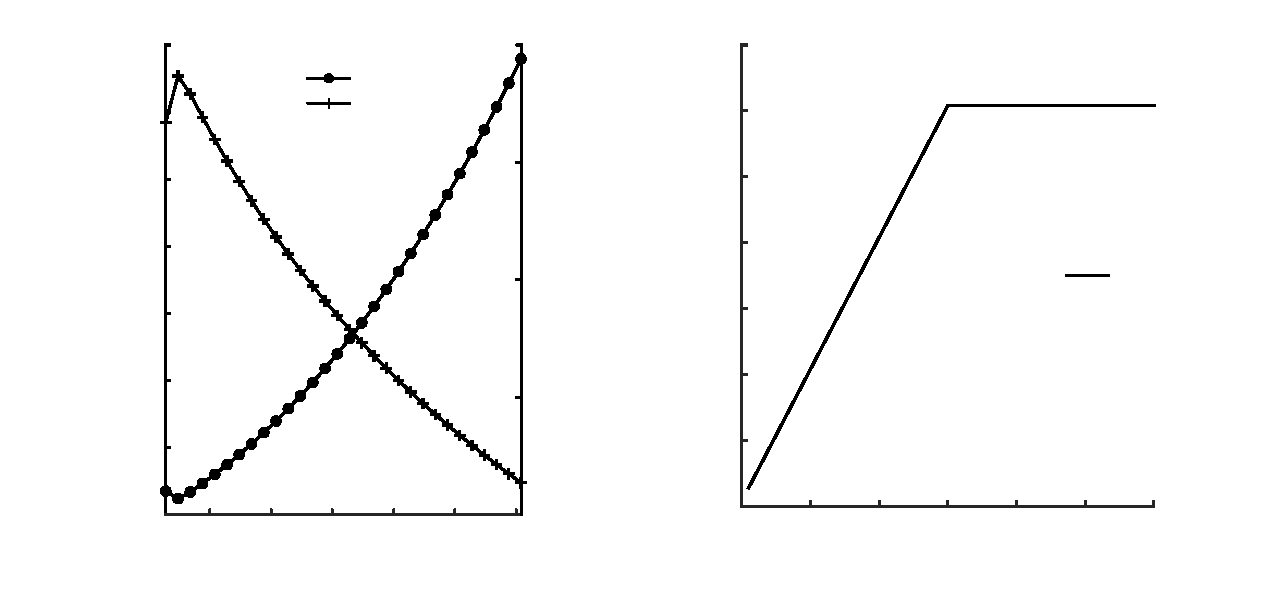
\includegraphics[scale=1]{diamtroDe3-inc}
\end{picture}%
\begin{picture}(612,288)(0,0)
\fontsize{8}{0}\selectfont\put(100.733,35){\makebox(0,0)[t]{\textcolor[rgb]{0.15,0.15,0.15}{{30}}}}
\fontsize{8}{0}\selectfont\put(130.14,35){\makebox(0,0)[t]{\textcolor[rgb]{0.15,0.15,0.15}{{35}}}}
\fontsize{8}{0}\selectfont\put(159.547,35){\makebox(0,0)[t]{\textcolor[rgb]{0.15,0.15,0.15}{{40}}}}
\fontsize{8}{0}\selectfont\put(188.954,35){\makebox(0,0)[t]{\textcolor[rgb]{0.15,0.15,0.15}{{45}}}}
\fontsize{8}{0}\selectfont\put(218.361,35){\makebox(0,0)[t]{\textcolor[rgb]{0.15,0.15,0.15}{{50}}}}
\fontsize{8}{0}\selectfont\put(247.768,35){\makebox(0,0)[t]{\textcolor[rgb]{0.15,0.15,0.15}{{55}}}}
\fontsize{8}{0}\selectfont\put(75.5703,41.0104){\makebox(0,0)[r]{\textcolor[rgb]{0,0,0}{{2}}}}
\fontsize{8}{0}\selectfont\put(75.5703,73.2089){\makebox(0,0)[r]{\textcolor[rgb]{0,0,0}{{4}}}}
\fontsize{8}{0}\selectfont\put(75.5703,105.407){\makebox(0,0)[r]{\textcolor[rgb]{0,0,0}{{6}}}}
\fontsize{8}{0}\selectfont\put(75.5703,137.606){\makebox(0,0)[r]{\textcolor[rgb]{0,0,0}{{8}}}}
\fontsize{8}{0}\selectfont\put(75.5703,169.804){\makebox(0,0)[r]{\textcolor[rgb]{0,0,0}{{10}}}}
\fontsize{8}{0}\selectfont\put(75.5703,202.003){\makebox(0,0)[r]{\textcolor[rgb]{0,0,0}{{12}}}}
\fontsize{8}{0}\selectfont\put(75.5703,234.201){\makebox(0,0)[r]{\textcolor[rgb]{0,0,0}{{14}}}}
\fontsize{8}{0}\selectfont\put(75.5703,266.4){\makebox(0,0)[r]{\textcolor[rgb]{0,0,0}{{16}}}}
\fontsize{8}{0}\selectfont\put(164.84,23){\makebox(0,0)[t]{\textcolor[rgb]{0.15,0.15,0.15}{{Diámetro de Tubería D 
[mm]}}}}
\fontsize{8}{0}\selectfont\put(62.5703,153.705){\rotatebox{90}{\makebox(0,0)[b]{\textcolor[rgb]{0,0,0}{{Caudal Q [L/s]}}}}}
\fontsize{8}{0}\selectfont\put(250.12,259.774){\makebox(0,0)[r]{\textcolor[rgb]{0,0,0}{{$D_e~\displaystyle\longrightarrow$ }}}}
\fontsize{8}{0}\selectfont\put(100.733,35){\makebox(0,0)[t]{\textcolor[rgb]{0.15,0.15,0.15}{{30}}}}
\fontsize{8}{0}\selectfont\put(130.14,35){\makebox(0,0)[t]{\textcolor[rgb]{0.15,0.15,0.15}{{35}}}}
\fontsize{8}{0}\selectfont\put(159.547,35){\makebox(0,0)[t]{\textcolor[rgb]{0.15,0.15,0.15}{{40}}}}
\fontsize{8}{0}\selectfont\put(188.954,35){\makebox(0,0)[t]{\textcolor[rgb]{0.15,0.15,0.15}{{45}}}}
\fontsize{8}{0}\selectfont\put(218.361,35){\makebox(0,0)[t]{\textcolor[rgb]{0.15,0.15,0.15}{{50}}}}
\fontsize{8}{0}\selectfont\put(247.768,35){\makebox(0,0)[t]{\textcolor[rgb]{0.15,0.15,0.15}{{55}}}}
\fontsize{8}{0}\selectfont\put(254.11,41.0104){\makebox(0,0)[l]{\textcolor[rgb]{0,0,0}{{0.014}}}}
\fontsize{8}{0}\selectfont\put(254.11,97.3578){\makebox(0,0)[l]{\textcolor[rgb]{0,0,0}{{0.015}}}}
\fontsize{8}{0}\selectfont\put(254.11,153.705){\makebox(0,0)[l]{\textcolor[rgb]{0,0,0}{{0.016}}}}
\fontsize{8}{0}\selectfont\put(254.11,210.053){\makebox(0,0)[l]{\textcolor[rgb]{0,0,0}{{0.017}}}}
\fontsize{8}{0}\selectfont\put(254.11,266.4){\makebox(0,0)[l]{\textcolor[rgb]{0,0,0}{{0.018}}}}
\fontsize{8}{0}\selectfont\put(277.11,153.705){\rotatebox{90}{\makebox(0,0)[t]{\textcolor[rgb]{0,0,0}{{Factor de Friccion $f$}}}}}
\fontsize{8}{0}\selectfont\put(250.12,56.2745){\makebox(0,0)[r]{\textcolor[rgb]{0,0,0}{{$f_e~\displaystyle\longrightarrow$ }}}}
\fontsize{8}{0}\selectfont\put(171.853,250.387){\makebox(0,0)[l]{\textcolor[rgb]{0,0,0}{{Q}}}}
\fontsize{8}{0}\selectfont\put(171.853,238.383){\makebox(0,0)[l]{\textcolor[rgb]{0,0,0}{{$f$}}}}
\fontsize{8}{0}\selectfont\put(356.062,39){\makebox(0,0)[t]{\textcolor[rgb]{0.15,0.15,0.15}{{0}}}}
\fontsize{8}{0}\selectfont\put(389.029,39){\makebox(0,0)[t]{\textcolor[rgb]{0.15,0.15,0.15}{{10}}}}
\fontsize{8}{0}\selectfont\put(421.995,39){\makebox(0,0)[t]{\textcolor[rgb]{0.15,0.15,0.15}{{20}}}}
\fontsize{8}{0}\selectfont\put(454.961,39){\makebox(0,0)[t]{\textcolor[rgb]{0.15,0.15,0.15}{{30}}}}
\fontsize{8}{0}\selectfont\put(487.927,39){\makebox(0,0)[t]{\textcolor[rgb]{0.15,0.15,0.15}{{40}}}}
\fontsize{8}{0}\selectfont\put(520.894,39){\makebox(0,0)[t]{\textcolor[rgb]{0.15,0.15,0.15}{{50}}}}
\fontsize{8}{0}\selectfont\put(553.86,39){\makebox(0,0)[t]{\textcolor[rgb]{0.15,0.15,0.15}{{60}}}}
\fontsize{8}{0}\selectfont\put(352.066,45.0106){\makebox(0,0)[r]{\textcolor[rgb]{0.15,0.15,0.15}{{25}}}}
\fontsize{8}{0}\selectfont\put(352.066,76.6376){\makebox(0,0)[r]{\textcolor[rgb]{0.15,0.15,0.15}{{30}}}}
\fontsize{8}{0}\selectfont\put(352.066,108.265){\makebox(0,0)[r]{\textcolor[rgb]{0.15,0.15,0.15}{{35}}}}
\fontsize{8}{0}\selectfont\put(352.066,139.892){\makebox(0,0)[r]{\textcolor[rgb]{0.15,0.15,0.15}{{40}}}}
\fontsize{8}{0}\selectfont\put(352.066,171.519){\makebox(0,0)[r]{\textcolor[rgb]{0.15,0.15,0.15}{{45}}}}
\fontsize{8}{0}\selectfont\put(352.066,203.146){\makebox(0,0)[r]{\textcolor[rgb]{0.15,0.15,0.15}{{50}}}}
\fontsize{8}{0}\selectfont\put(352.066,234.773){\makebox(0,0)[r]{\textcolor[rgb]{0.15,0.15,0.15}{{55}}}}
\fontsize{8}{0}\selectfont\put(352.066,266.4){\makebox(0,0)[r]{\textcolor[rgb]{0.15,0.15,0.15}{{60}}}}
\fontsize{8}{0}\selectfont\put(339.066,155.705){\rotatebox{90}{\makebox(0,0)[b]{\textcolor[rgb]{0.15,0.15,0.15}{{Diámetro de Tubería D [mm]}}}}}
\fontsize{8}{0}\selectfont\put(454.961,27){\makebox(0,0)[t]{\textcolor[rgb]{0.15,0.15,0.15}{{Número de
iteraciones
en el lazo for}}}}
\fontsize{8}{0}\selectfont\put(527.487,249.954){\makebox(0,0)[r]{\textcolor[rgb]{0,0,0}{{Convergencia de D}}}}
\fontsize{8}{0}\selectfont\put(535.847,155.705){\makebox(0,0)[l]{\textcolor[rgb]{0,0,0}{{D}}}}
\fontsize{10}{0}\selectfont\put(104.04,5.76001){\makebox(0,0)[l]{\textcolor[rgb]{0,0,0}{{(a) Q y $f$ en función de D}}}}
\fontsize{10}{0}\selectfont\put(364.14,5.76001){\makebox(0,0)[l]{\textcolor[rgb]{0,0,0}{{(b) D en función del número de iteraciones}}}}
\end{picture}
\end{document}
